\chapter{\statusorange Related Work}
\label{chap:literature}

In this chapter, we present the state of the art for the different research areas that we plan to touch in the next chapters. Each of the sections is related to one of the Research Questions presented in the previous chapter.

We start from the literature targeted to analysing similar articles (Section~\ref{sec:lit_relationships}), which considers relationships and similarities between different documents.
Then we move to the literature about persuasion detection, especially focusing on sentiment and propaganda detection (Section~\ref{sec:lit_persuasion}).
Next, we describe the literature about political leaning, describing the definitions and the approaches for the automatic classification (Section~\ref{sec:lit_leaning}).
And finally, we present the works on topic recognition, giving an overview of the existing approaches (Section~\ref{sec:lit_topics}).

\todo{Other related phenomena? Remove or introduce here}

After this overview of each of them, we discuss the limitations of not considering these research areas together, and the potential benefits of performing comparative analysis across dimensions (Section~\ref{sec:lit_discussion}).

To conclude, we present the scope of this work in Section~\ref{sec:lit_scope}.


% Similarity and parallel news

% \gls{propaganda}

% - Propaganda and misinformation

% \Gls{political-leaning}: definitions/classification

% topics

\section{\statusgreen Similarity between articles}
\label{sec:lit_relationships}

Our starting point is the literature that aims at analysing multiple versions of the same story, across different news sources.

From the enormous multitude of articles that get published every day, several datasets and resources of parallel news have been built (described in Subsection~\ref{ssec:lit_relationships_parallel}.
We are interested in works that explore what changes between similar articles, and the literature defines and deals with different tasks (Subsection~\ref{ssec:lit_relationships_tasks}). We focus specifically on corroboration and omission detection (Subsection~\ref{ssec:lit_relationships_corr_omiss}.

\subsection{Parallel News}
\label{ssec:lit_relationships_parallel}

To talk about similarity between news articles we first need to introduce the concept of \emph{\gls{parallel-news}}

\emph{Parallel corpus} is a term that is frequently utilised when multiple languages are involved.
These resources, such as the OPUS dataset~\citep{tiedemann2012parallel}, are useful for applications in computational linguistics, translation studies and cross-linguistic corpus studies~\citep{brown1991aligning,ramesh2022samanantar,ziemski2016united,kunchukuttan2017iit,banon2020paracrawl}.

We take the usage of this term in a monolingual setting, where each document contains a certain number of variations from the others, but still covers the same main events.
This specific connotation is considered in works that perform sentence-level paraphrase extraction~\citep{dolan2004unsupervised,zhang2013harvesting}.
More specifically in the news media environment, several datasets and tools have been developed with the aim of exposing the users to several points of view~\citep{bozdag2015breaking}, in order to break the filter bubble~\citep{pariser2011filter} that is built around them.

Some resources just group together news articles that are related, such as news aggregators, like Google News with the feature \emph{Full Coverage},\footnote{\url{https://blog.google/products/news/new-google-news-ai-meets-human-intelligence/}} that presents a collection of articles for each headline.
There are also resources that try to bring together opposing points of view, such as Allsides Headline Roundup,\footnote{\url{https://www.allsides.com/headline-roundups}} or research works that try to provide a similar result~\citep{trampuvs2015diversinews,park2009newscube}.


% \cite{bountouridis2018explaining}

Some of these resources are hand-curated while others are algorithmically synthesised. In the hand-curated groups (e.g., AllSides), there are usually domain experts or editors who manually put together news articles that share the same events and details. With AllSides, the editors select one article from the Left, one from the Center and one from the Right to ensure that different sides of the story are presented.
Instead, with algorithmic resources (e.g., Google News Full Coverage), there is an automated approach that, based on clustering algorithms, creates groups of articles that cover the same story~\citep{marutho2018determination,alelyani2018feature,karimi2018news}.

\subsection{Common Tasks}
\label{ssec:lit_relationships_tasks}

With this availability of resources, both in the news domain but also with a wider perspective, the computational linguistics community has identified and targeted several tasks.

First of all, we need to mention the \textit{semantic similarity} task.
Semantic similarity is defined as the likeness of meaning or semantic content as opposed to lexicographical similarity, which instead relies more on the exact terms matching~\citep{harispe2015semantic}.
The research community has created different benchmarks to evaluate models on their ability to capture the semantic similarity~\citep{conneau-kiela-2018-senteval,chandrasekaran2021evolution}.
As for what discerns the models, we have had an evolution over the last years, starting from the first generations of word embeddings~\citep{pennington2014glove,mikolov2013efficient}, up to the recent family of transformers-alike models~\citep{devlin2018bert,cer2018universal,yang2019xlnet,reimers2019sentence}.

We then find another task that exploits similar ideas: \emph{finding related claims}~\citep{almeida2020text}.
This task is extremely useful for works that try to estimate the truthiness of claims, by looking for similar claims that have already been verified or refuted. This process is used as the first step in automated fact-checking~\citep{nakov2021automated,guo2022survey}. This task is particularly challenging because small changes (e.g., a number reported or a negation) can drastically change the truthiness of a sentence.


% Suggest items to read (recommender systems)
Another task that relies on semantic similarity, is the recommendation of content (e.g., news articles) that is similar to a reference one.
This opens the immense field of recommender systems~\citep{tintarev2006similarity,karimi2018news,feng2020news}, where there may be more than one objective function to satisfy.
Besides semantic similarity, the alignment with the point of view of the reader is important (but needs to be limited to avoid the filter-bubble effect)~\citep{lunardi2020metric,nguyen2014exploring,lunardi2019representing}.
Or also the serendipity~\citep{ziarani2021serendipity,abdollahpouri2021toward,raza2022news} of recommendations.

Lastly, we can also consider as related the \emph{plagiarism detection} task.
In this task, the goal is to spot fragments of text that have been copied from others, without reference or with a certain proportion~\citep{stein2006near,alzahrani2010fuzzy,arabi2022improving}.


\subsection{Corroboration and Omission Detection}
\label{ssec:lit_relationships_corr_omiss}

The task that instead we focus on with this work, is the investigation of \textit{corroboration and omission} across multiple sources.
This task focuses on comparing and contrasting similar articles, to find which parts are in common and which ones are omitted~\cite{ehrhardt2021omission,bountouridis2018explaining,ko2023claimdiff}.
By analysing multiple news articles it becomes possible to understand the interrelationships between multiple points of view.

For example, \cite{bountouridis2018explaining} extracts points of information in all the articles, cross-compares them across groups of related articles, and is able to detect which details are corroborated in multiple sources and which ones instead are omitted.
Then the authors follow with a source-based aggregation and build indicators of credibility. The rationale is that corroborating a detail with external sources indicates that the detail is more likely to be true.
Instead, if a news source omits a detail that other sources mention, it is a potential negative sign.
Therefore, the more corroboration and the less omission a news source contains, the more credible it is.
The approach is validated by showing a positive correlation between these indicators and the values of credibility retrieved from Media Bias/Fact Check.\footnote{\url{https://mediabiasfactcheck.com/}}

\subsection{Limitations}
% What is missing?

% Fine-grained study of the terms that change $\rightarrow$ our goal to expand
From these works on corroboration and omission detection, we find it limiting that the analysis is performed only considering points of information/details but not the single words involved.
Once the details are identified across articles, it would be very useful to analyse the slight variations in terms.
For example, it could be possible to identify terms that are unique and terms that instead are used across multiple sources. By bringing this analysis to the word level, we can be more specific.
We will expand on this in Chapter~\ref{chap:common_ground_search}, where we address this limitation together with other limitations (e.g., semantic similarity models used, more resistant to term changes).

% What the term choice may mean (persuasion) $\rightarrow$ using literature on persuasion, considering multiple research areas together 
The next big limitation that we find, is that it would be very important to go beyond the single analysis of similarities, and study what these changes involve.
For this reason, in our work we also explore other related dimensions, such as persuasion.
Our aim is to see how the variations between multiple articles (specific term choices) cause changes in detected persuasion. In other words, what is the effect of using one term instead of a synonym that may carry an additional load?


% From the existing literature, we find that there are certain limitations that come from only analysing similarity
This type of limitation can be overcome only with a study that involves multiple factors at the same time, like a comparative analysis.

\section{\statusorange Persuasion detection}
\label{sec:lit_persuasion}

The next research area that we are touching in our work is \emph{persuasion detection}.
We are interested in getting an understanding of what words convey, beyond the simple expression of content.
We want to have an additional study of what specific choices (terms, details, order of presentation) may convey.

% Before describing the literature, we need here to present our motivation for introducing this research topic. 


Contextualising in the current attention economy~\citep{davenport2001attention}, recent literature sees a rise in the race for attention also in news articles, characterised by the emergence of clickbaitness and language that is increasingly more loaded ~\citep{bazaco2019clickbait,davenport2001attention}.
With the enormous amount of news sources and news articles covering the same events, it is very important for news sources to compete for the clicks and reads of the consumers.

Persuasion is generally defined as a method to ``influence a person's beliefs, attitudes, intentions, motivations, or behaviours"~\cite{gass2018persuasion}.
We see several related concepts in the literature that can be considered as forms of persuasion:
\begin{itemize}
    \item sentiment overloading: using emotional language to convey strong emotions to the reader; % loaded language instead?
    \item \gls{propaganda}:  information, ideas, opinions, or images, often only giving one part of an argument, that are broadcast, published, or in some other way spread with the intention of influencing people's opinions\footnote{\url{https://dictionary.cambridge.org/dictionary/english/propaganda}} % to indoctrinate a population towards an individual or a particular agenda
    \item \gls{populism}: political ideas and activities that are intended to get the support of ordinary people by giving them what they want\footnote{\url{https://dictionary.cambridge.org/dictionary/english/populism}}
    \item coercion: the use of force to persuade someone to do something that they are unwilling to do\footnote{\url{https://dictionary.cambridge.org/dictionary/english/coercion}} % aggressive threats and the provocation of fear and/or shame to influence a person's behavior.
\end{itemize}

Across these multiple forms, we explore in a more detailed way the first two: sentiment and propaganda.
Persuasion is linked with sentiment because of its goal to influence the emotional response~\citep{gatti2014sentiment,rocklage2018persuasion,petty2015emotion,desteno2004discrete}.
Instead, the relationship with propaganda comes from the inherent goal of propaganda to influence the public's view about an idea or a group~\citep{bernays,jowett2018propaganda}.

We dedicate the following two subsections to sentiment and propaganda detection respectively.

\subsection{\statusgreen Sentiment Analysis}
\label{sec:lit_sentiment}


Sentiment analysis is the computational treatment of opinions, sentiments and subjectivity of text~\citep{medhat2014sentiment}.
Several surveys have been published in the recent years~\citep{liu2010sentiment,medhat2014sentiment,wankhade2022survey}, and we rely on them to examine the tasks and techniques available.


% liu2010sentiment,medhat2014sentiment,wankhade2022survey : surveys

The first broad distinction that we need to make, is the granularity of the analysis.
Starting from the widest, we have \emph{document-level} classification, which means assigning to a whole document a single output.
Then, other approaches define the \emph{sentence-level} classification, which instead provides for each sentence an output. In this way, it is possible to analyse the evolution of the sentiment across a document, and get more detailed information.
And the more detailed analyses provide \emph{aspect-level} classification~\citep{zhang2022survey}. In this case, we get an analysis of each aspect mentioned in the document. An aspect can be an entity or even a feature of an object (e.g., colour, shape) and in this way, we can have an output that is very much related to single words.

The second distinction is based on the techniques used for the analysis. There are several techniques that range from simple dictionary-based to advanced deep-learning techniques.
The ones that have a longer history are the family of \emph{lexicon-based} models~\citep{taboada2011lexicon}. Being the simplest and most intuitive, there are many of them that are still very popular today. Even new models belonging to this family keep being developed, as it is a very powerful technique.
In this family, there are two subtypes: dictionary-based and corpus-based.
% https://www.sciencedirect.com/science/article/pii/S2090447914000550
Dictionary-based models depend on sentiment-carrying words that are used as seeds, and then search the dictionary for their synonyms and antonyms. In this way, large lists of words together with their sentiment are built~\citep{okango2022dictionary,hardeniya2016dictionary}.
Corpus-based models also start with seed terms, but then do the expansion with a corpus looking for synonyms, using statistical or semantic methods~\citep{darwich2019corpus,rice2021corpus}.

% They are built around a lexicon where each word has a specific score, and some combination rules. But we do not exclude tools that work with a different, more complex approach. It is only required from them to give a score specific to the individual words. 

From this family of approaches, we also have very popular tools that can be used freely, such as Sentistrength\footnote{\url{http://sentistrength.wlv.ac.uk/}}, Vader\footnote{\url{https://github.com/cjhutto/vaderSentiment}} and TextBlob.\footnote{\url{ https://textblob.readthedocs.io/}}


Instead, more advanced models are based on machine learning (mostly supervised, but also some unsupervised).
In the supervised approaches, we find examples of decision trees, SVM, rule-based classifiers, Naive Bayes, Bayesian Networks, and Maximum Entropy approaches~\citep{zharmagambetov2015sentiment,bayhaqy2018sentiment,fitri2019sentiment,rathi2018sentiment,xie2019improved}.
The more recent ones rely on Deep-Learning models~\citep{zhang2018deep}, where there are multiple combinations considering:
\begin{itemize}
    \item document encoding: Bag of Words~\citep{moraes2013document,zhai2016semisupervised}, word embeddings~\citep{tang2015document,chen2016neural}, dense document vectors~\citep{le2014distributed}
    \item network architectures: feed-forward~\citep{duncan2015neural}, autoencoders~\citep{zhai2016semisupervised,wu2019semi}, CNN~\citep{jianqiang2018deep,sun2019aspect}, recurrent~\citep{chen2017recurrent,xu2016cached}, recursive~\citep{wang2016recursive,nguyen2015phrasernn}, memory networks~\citep{li2017end,lv2021aspect}
    \item attention mechanism: no attention, hierarchical~\citep{zhou2016attention}, sequence, alignment
\end{itemize}



% Techniques of detection: (medhat2014sentiment)
% - lexicon-based
%   - dictionary-based
%   - corpus-based
%     - statistical
%     - semantic
% - ML-based
%   - supervised
%     - decision tree classifiers
%     - linear classifiers (SVM/Neural Networks)
%     - rule-based classifiers
%     - probabilistic classifiers (Naive Bayes, Bayesian Network, Maximum Entropy)
%     - Deep Learning (zhang2018deep survey):
%       - Document-Level classification
%         - Document representation: BoW, word embeddings, dense document vector
%         - Neural Network Model: Feedforward Neural Network, Autoencoder, CNN, Recurrent/LSTM/GRU, Memory Network
%         - Attention: No, Hierarchical, 
%       - Sentence-Level Classification
%         - Same as Document-level
%         - Adding: parse trees, opinion lexicons, and part-of-speech tags
%         - CNN/RNN: semantic and syntactic information from word embeddings
%       - Aspect-based Classification: Context, Target Representation, Sentiment Context (done with attention)
%   - unsupervised
%     - game theory
%     - based on sentiment clustering
%     - generative-model based: asking GPT-similar models, context of classification

% zhang2018deep : deep learning for sentiment analysis
% godbole2007large : large scale sentiment analysis

From this large group of publication and approaches, the solutions are less democratised, which means that it is usually very hard to reproduce the models and results, because of non-shared code-bases, datasets and parameters.
This means that there are less publicly available tools that perform this type of analysis.
One of the few exceptions is Stanford CoreNLP which is based on a RNN~\citep{socher2013recursive} that accounts for the sequence but also for the dependency tree of the sentence (in other words, discovering the combination rules autonomously). It is based on a dataset that links sentiment scores to a dependency tree (Sentiment Treebank\footnote{\url{https://nlp.stanford.edu/sentiment/treebank.html}}).

If at first glance, the advanced deep learning models may seem more reliable, we find that the most robust and common methods are the simpler ones.
We have recent examples of lexicon-based approaches~\citep{okango2022dictionary,mitra2020sentiment}.
And especially in combination with aspect-based detection, we see that the status is yet in an exploratory phase, without major shared tools being built.

\subsection{\statusorange Propaganda}
\label{sec:lit_propaganda}

Moving instead to \emph{propaganda}, we can start with some theoretical definitions.
According to~\cite{jowett2012propaganda}, ``propaganda  is  a  form  of  communication  that  attempts  to  achieve a  response  that  furthers  the  desired  intent  of  the  propagandist." This is slightly different from persuasion, which instead is ``interactive and attempts to satisfy the needs of both persuaded and persuadee."  %A  model  of  propaganda  depicts  how  elements of  informative  and  persuasive  communication  may  be  incorporated into  propagandistic  communication,  thus  distinguishing  propaganda as  a  specific  class  of  communication.  References  are  made  to  past theories  of  rhetoric  that  indicate  propaganda  has  had  few  systematic theoretical  treatments  prior  to  the  20th  century.  Public  opinion  and behavioral change can be affected by propaganda.
% The terms propaganda and persuasion have been used interchangeably in the literature on propaganda, as well as in everyday speech. Propaganda employs persuasive strategies, but it differs from persuasion in purpose.





% TODO propaganda definition in different fields.

% First of all, let us start with a definition of propaganda.
We can then consider the definition from the Cambridge Dictionary, which defines propaganda as the use of language ``with the intention of influencing people's opinions."\footnote{\url{https://dictionary.cambridge.org/dictionary/english/propaganda}}
It has many points in common with argumentation and rhetorics and is usually associated with deceiving techniques, partial point of views, logical fallacies.
In his book on propaganda, Edward Bernays defines it as a ``consistent, enduring effort to create or shape events to influence the relations of the public to an enterprise, idea or group''~\cite{bernays}.

Propaganda possesses unique characteristics that go beyond its ability to persuade. It typically targets a significant audience, promotes the agenda of a particular group, and employs flawed reasoning and/or emotional appeals~\cite{miller1939techniques}.

Injecting propaganda into the political narrative is an old and common tactic to influence opinions and push certain ideologies or agendas.
Propaganda can more practically be defined as the usage of a set of techniques. These techniques vary from the usage of emotional language (e.g. loaded language, appeal to fear) to logical fallacies (bandwagon, red herring).

Propaganda is very related to the agenda-setting theory \citep{Cohen_1964,mccombs1972agenda}, which describes the ability of news media to influence the importance placed on the topics of the public agenda.

Over the next paragraphs, we first give more theoretical background about the \emph{propaganda model}, which describes the way that propaganda acts on society.
Afterwards, we give an oversight to the most common propaganda techniques.
To conclude, we present some works that try to detect propaganda at different granularities.

\subsubsection{The Propaganda Model}

According to the propaganda model, which was developed by~\citet{herman1988manufacturing}, corporate mass media functions based on propaganda and systemic biases. It explains how populations are manipulated, and how consent for economic, social, and political policies is manufactured through propaganda. Media structures that create inherent conflicts of interest (e.g. advertising, media concentration, government sourcing) act as propaganda for anti-democratic forces, according to the theory.
The theory relies on five \emph{filters} that determine the type of news that is presented in the media:

% the problem is X taken from phillips2007left https://www.projectcensored.org/wp-content/uploads/2010/05/LeftProgressiveMediaInsideth_PropagandaModel.pdf
\begin{enumerate}
    \item Ownership: since the mainstream media outlets are usually big conglomerates, there will be some bias toward their interests in the information presented. The problem is the concentrated private ownership.
    \item Advertising: the news is only a ``filler" to post advertisements, and therefore it needs to align with the ``buying mood". The problem is the orientation to profit.
    \item Sourcing: first-hand news comes mostly from officials and powerful sources, because it is not affordable to have reporters everywhere. The problem is the over-reliance on governmental and corporate sources for news.
    \item Flak: negative responses to the media statements or programs, such as complaints and other actions that are performed by organizations and coalitions, to disagree or to discredit. The problem is the tendency to avoid offending the powerful.
    \item Fear: anti-ideologies (e.g. anti-communism historically, anti-terrorism) that exploit public fear of groups that are potentially a threat. The problem is religiously following the mainstream ideas, and strongly opposing alternative beliefs.
\end{enumerate}

These five filters together set what is considered acceptable in the coverage of daily events~\citep{phillips2007left}. ``Newsworthy" criteria influences journalists and editors, and everything that diverges from the ``common sense" is self-disciplined and self-censored.

While the model primarily draws from U.S. media, Chomsky and Herman assert that the theory can be extended to any nation with similar fundamental economic and organizational foundations, as outlined by the model, which contribute to the emergence of media prejudices. This viewpoint has garnered support from various scholars, and investigations into the media's propagandistic functions have subsequently been conducted and validated in Western Europe and Latin America~\citep{herman1996propaganda}.


\subsubsection{Propaganda techniques (computational)}

If we look at more practical definitions of propaganda, we see that in the literature several works have addressed propaganda as a set of techniques~\citep{torok2015symbiotic,miller1939techniques,weston2018rulebook}. The recent work of~\citet{da2019fine} takes from these works and considers only the techniques that can be found in journalistic articles and that can be judged intrinsically without needing external evidence.

These techniques are:
\begin{enumerate}
    \item Loaded language:
    \item Name calling or labelling:
    \item Repetition: Exaggeration or minimisation:
    \item Doubt:
    \item Appeal to fear/prejudice:
    \item Flag-waving
    \item Causal oversimplification:
    \item Slogans: 
    \item Appeal to authority: 
    \item Black and white fallacy:
    \item Thought-terminating cliché:
    \item Whataboutism: 
    \item Reductio ad Hitlerum: 
    \item Red herring: 
    \item Bandwagon: 
    \item Obfuscation, intentional vagueness, confusion: 
    \item Straw man: 
\end{enumerate}

\todo{continue from here, fill description of techniques above}


\subsubsection{Propaganda detection (computational)}
\label{ssec:lit_propaganda_detection}


% FROM TTO21
%\subsection{Propaganda}
%\label{ssec:related_prop}

% In his book on propaganda, Edward Bernays defines it as a ``consistent, enduring effort to create or shape events to influence the relations of the public to an enterprise, idea or group''~\cite{bernays}.
% Injecting propaganda in the political narrative is an old and common tactic to influence opinions and push certain ideologies or agendas. However, to the best of our knowledge, current research on political leaning detection largely overlooked the direct inclusion of propaganda as analysis features in their computational models. 

Developing computational methods to detect the use of propaganda in text is very recent, and is primarily fuelled by the increased use of propaganda in misinformation dissemination \citep{da2020survey}. Most related work is limited to binary detection of propaganda (i.e. propaganda exists/does not exist) in general (i.e. regardless of propaganda technique), using n-gram logistic regression and SVM methods ~\citep{rashkin2017truth,barron2019proppy}. More recently, \citet{da2019fine} used a neural network approach to identify the text fragments that contain propaganda, and the particular propaganda techniques used (Figure~\ref{fig:propaganda_example_1}).


%On this, we have our hypothesis that \emph{we can recognise the political leaning of an article by using the features provided by the propaganda analysis}.
%The mixed analysis would allow to understand better why a certain article is classified as being left/right with respect to the black box BERT classifier.


%On the other side, we are considering the use of language that is targeted to push for a certain political view. There are many linguistic choices and devices, along with how the narrative is structured, that are used to promote a specific viewpoint.
%Propaganda is defined as something that can be recognised by its persuasive function, sizeable target audience, the representation of a specific group’s agenda, and the use of faulty reasoning and/or emotional appeals~\cite{miller1939techniques}. The list of such techniques is very long\footnote{\url{https://en.wikipedia.org/wiki/Propaganda_techniques}}, and here we are considering the ones that have been analysed automatically by~\citet{da2019fine}. The propaganda is the most persuasive/loaded part of an article.
% \item sentiment usage: loaded language in the articles can reveal strong subjectivity against the mentioned entities. This relates to the subjective part of articles and we want to take this into consideration
% \item narrative/persuasion and other related analyses?

\begin{figure}[!htb]
    \centering
    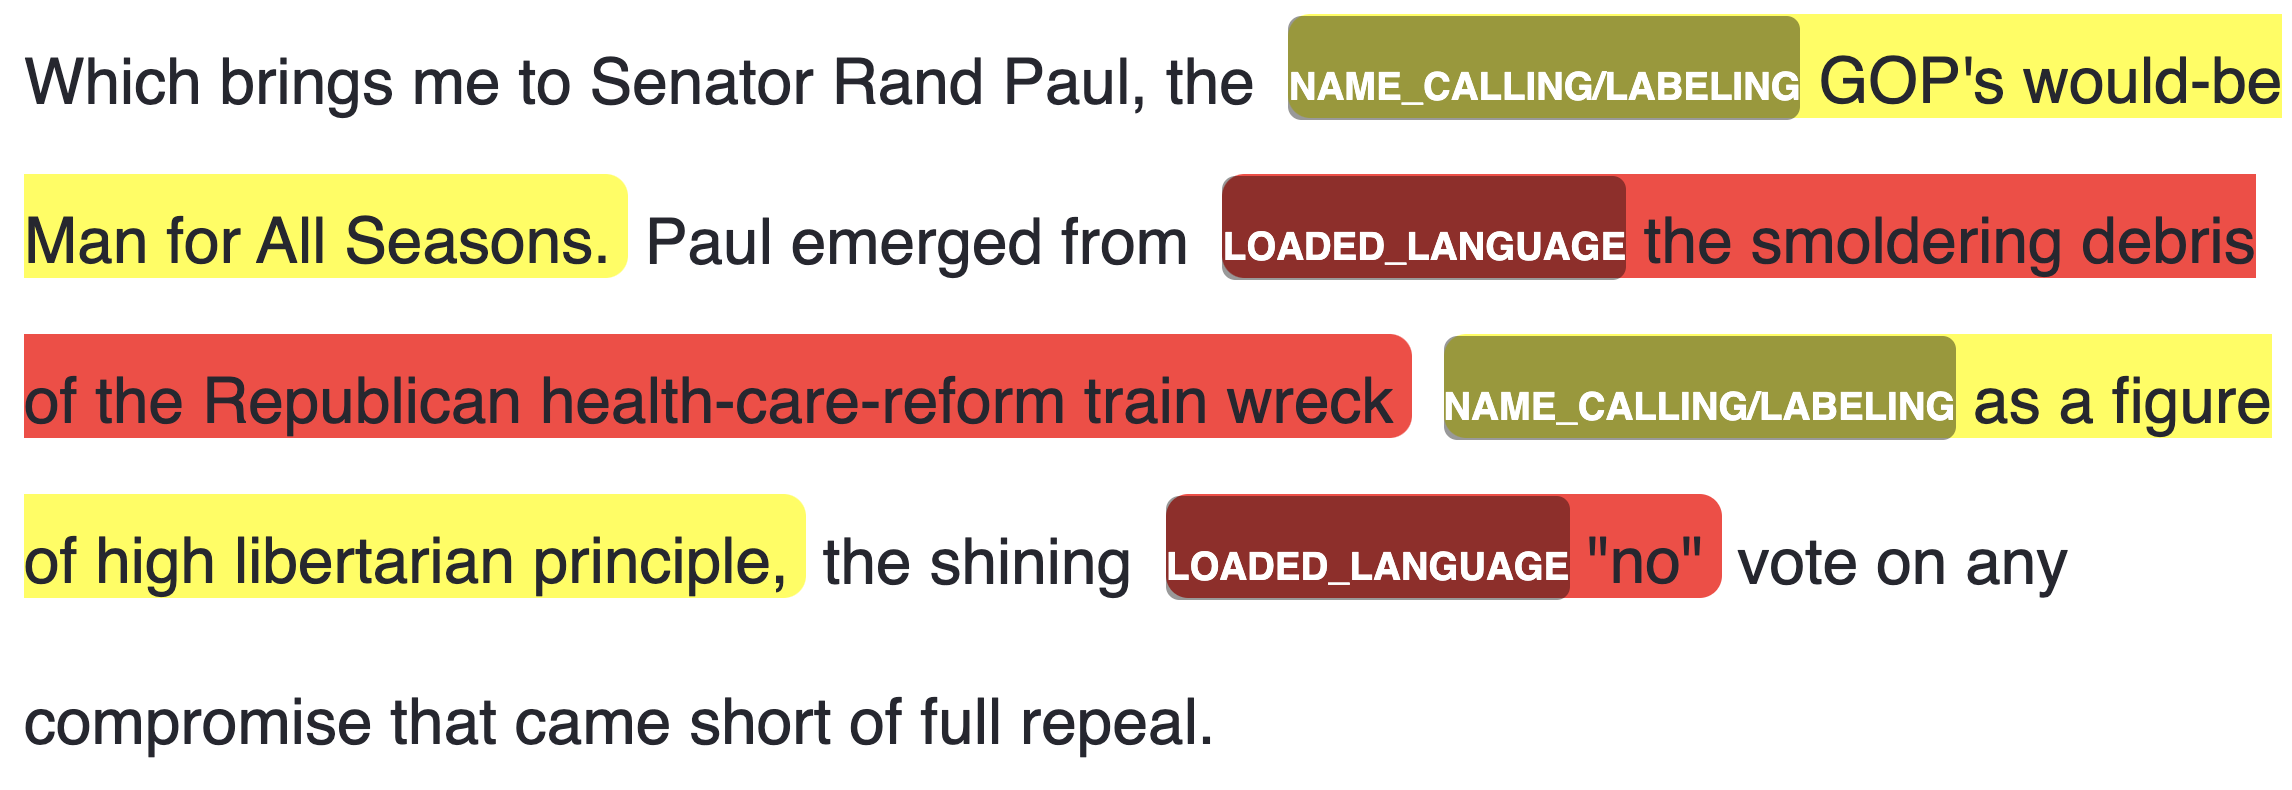
\includegraphics[width=\linewidth]{figures/propaganda_example_1_color.png}
    \caption{Detection of propaganda techniques using~\citet{baly2020we}.% the article comes from NationalReview, a source with Right-leaning bias.
    }
    \label{fig:propaganda_example_1}
\end{figure}


%For the propaganda analysis, we are focusing on the computational propaganda, defined as the propaganda that has been analysed by computational approaches. 
%The survey conducted by~\citet{da2020survey} displays the most important works, and also underlines the main limitation of current methods.
%The biggest limitation that we see, is that \emph{explainability is a desirable feature} but current approaches do not provide it.
%Most of the models only classify full articles as being propagandist or not~\cite{barron2019proppy,rashkin2017truth}, and this does not help to understand why.
%Therefore, another work focuses on fine-grained techniques~\cite{da2019fine}: every article analysed is annotated with labels coming from 18 different techniques, also indicating the spans affected by the techniques. So we can see where propaganda is inside an article and which specific techniques were used. Figure~\ref{fig:propaganda_example_1}

TODO: The datasets for detection: article-level, fine-grained

\subsection{\statusred Limitations}
HERE?

\subsection{\statusgreen Layers of information}
\label{ssec:lit_layers_of_info}
We see this as text conveying two layers of information:
\begin{enumerate}
    \item the first layer, the most visible, is the layer of \emph{facts}: entities (what/who is mentioned) and actions (what happens), combined into events
    \item a second layer of additional and subjective information: choice of terms to use, details to include and exclude, order of presentation, expression of opinion, subjective statements. All these means are used to convey a certain point of view, and therefore we use the umbrella term of \emph{persuasion}.
\end{enumerate}


% Talk here about different layers: 1 facts, 2 persuasion ( propaganda/argumentation/sentiment). Or in other terms: topical and non-topical elements.

These two layers can be more or less intertwined, and it can become more difficult to distinguish between them.
In the easiest cases, they can be identified on the linguistic surface of different words: some words in a sentence that belong to the \emph{facts} layer (e.g., a name) accompanied by other words that belong to the \emph{persuasion} layer (e.g., an adjective).
In this case, it is conceptually easy to separate the two components in a text and say which word belongs to one or the other.

But in many other cases, the two components can also coexist within the same word. For example, a term may have been chosen both to communicate a certain concept (facts layer), but between many available terms, the author voluntarily or involuntarily picks one or another term that conveys a different opinion on the concept itself (persuasion layer).

% e.g. name+adjective, where the name is the topical element while the adjective can express the opinion of the writer (commenting, denigrating, complimenting, subjective).
% Or they can also be expressed in the same word together: this is where word selection applies. For example, when the writer needs to find a word for communicating a certain concept ``?", they can choose whether to use X or Y. While these two words have the same underlying concept, they express it quite differently.

% Or also called: Topic model and Anti-topic model (expand on this, as discussed during the upgrade)

% Propaganda: Communication with the goal to persuade

Our hypothesis is that \emph{we can distinguish between the two layers}.

We will discuss this hypothesis in Chapter~\ref{chap:linguistic_persuasion}


\section{\statusred Political Leaning}
\label{sec:lit_leaning}

\todo{Continue here to take all citations from Chapters 5-6 and expand on them}

Here in this section, we focus on the concept of Political Leaning.

First, we give a definition, and then we focus on the Political Leaning Classification task and how it has been addressed by the literature.

\subsection{Political Leaning Definition}

Political Leaning is a term that is derived from Political Ideology~\citep{jost2009political}.
Political ideology is defined as a ``set of beliefs about the proper order of society and how it can be achieved"~\citep[p.~64]{erikson2015american}.

From the multi-dimensional diversities in political ideologies, there is a historical tendency to consider only the Left-Right dimension~\citep{jost2009political}.
Although this simplification does not capture completely the complexity of determining one's political ideology, it is the most common way of describing political orientation.
Since only one dimension is considered, it is usually named as a political leaning or political spectrum.

% historical left and right

% https://www.dictionary.com/e/politics/political-spectrum/
% https://en.wikipedia.org/wiki/Political_spectrum
Historically, the usage of left and right originate during the 1789 French Revolution. The physical position of the politicians in the French National Assembly was that the revolutionaries were sitting together on the left side, while the aristocracy-favouring was on the right.\footnote{\url{https://www.dictionary.com/e/politics/political-spectrum/}}
Therefore, the newspapers started using the terms to mention respectively the liberal (left) and the authoritarian on the right.

From originally only two labels, in 1857 we have the first appearance (on the Southern Trade magazine) of the term \emph{political spectrum} to describe the range of political opinions.


% US and conservative vs liberal
% https://pleeps.org/en/wp-content/uploads/Political-Ideology-Its-Structure-Functions-and-Elective-Affinities.pdf (jost2009political)
The use of ``liberal" and ``conservative" as substitutes for ``left" and ``right" is becoming more prevalent in the United States and other countries.
This terminology effectively captures the historical ideological division between desires for change and stability.
These two desires, change vs maintaining the status-quo, are coming from debates that have their roots in age-old disputes regarding the appropriate levels of hierarchy, authority, and inequality~\citep{bobbio1996left}.


% https://pleeps.org/en/wp-content/uploads/Political-Ideology-Its-Structure-Functions-and-Elective-Affinities.pdf (jost2009political)
This formulation of the distinction between left and right is characterised by
two different aspects~\citep{jost2018political}:
\begin{itemize}
    \item supporting vs opposing social change
    \item rejecting vs accepting inequality
\end{itemize}
The most common terms that people from both left and right associate with the right are: “conservative,” “system maintenance,” “order,” “individualism,” “capitalism,” “nationalism,” and “fascism,” and they associated the left with “progressive,” “system change,” “equality,” “solidarity,” “protest,” “opposition,” “radical,” “socialism,” and “communism”~\citep[p.~213-14]{fuchs1990}.
The two core components of the left-right dimension, attitudes towards change versus stability, and equality versus inequality, are connected due to historical factors, as Western societies have gradually become more egalitarian over the past few centuries in terms of human rights and liberties, economic distribution, and political power distribution.
Equality has increased in some instances due to revolutionary events, which were frequently resisted or opposed by conservatives and those associated with the right~\citep{nosek2009politics,burke1790reflections}.



% automated paragraphs
Left-leaning ideologies are typically associated with progressive and socialist ideas, such as the belief in social equality, the importance of government intervention in economic matters, and the provision of public services.
Right-leaning ideologies, on the other hand, tend to prioritize individualism, capitalism, and free markets, with less emphasis on government intervention and regulation.

However, the specific meaning of left and right can vary across countries and political systems.
For instance, in some countries, left-wing political parties may advocate for more social welfare programs and nationalized industries, while in others, they may focus on issues such as civil liberties and human rights.
Similarly, right-wing parties may prioritize issues such as nationalism, religious conservatism, or economic liberalism, depending on the country's culture and political history.

Furthermore, the labels ``left" and ``right" can also be influenced by the particular issues and events of a given time period.
For example, in some countries, environmentalism and climate change have become important political issues that may cut across traditional left-right divides.
Similarly, issues such as immigration, trade, and national security may be more salient in certain countries than in others, shaping the way that people identify with different political ideologies.




% practical definition: view on issues
As a more practical and operable definition, we can define political leaning from the common positions that left and right have on issues such as economics, social policies, and governance.

% Position of the left and right (wikipedia/allSides):

% https://www.allsides.com/media-bias/rate-your-bias
\begin{table}[ht]
    \centering
    \begin{tabular}{p{0.2\linewidth} | p{0.4\linewidth} | p{0.4\linewidth}}
      Topic  & Left & Right \\ \hline
      Social issues & \\
      Abortion & rights of the mother, ability to have abortion & rights of the fetus, limiting and stopping abortions \\
      Gay marriages & no difference with opposite-sex couples & marriage between man and woman, gay marriage is different from what God intended \\
      Family & expanded view on non-traditional families & not encouraging divorced/single/unmarried parents (accepting them may be fine) \\
      Sexual and Gendered behaviour & accepting and empathetic culture & \\
      Sexuality & free expression is a right & \\
      TODO finish
    \end{tabular}
    \caption{Left and Right positions according to AllSides}
    \label{tab:allsides_leaning_positions}
\end{table}

Table~\ref{tab:allsides_leaning_positions} shows how AllSides recaps the common positions about different issues.\footnote{\url{https://www.allsides.com/media-bias/rate-your-bias}}.




\subsection{Political Leaning Classification}
\label{ssec:lit_leaning_classification}

FROM TTO2020

%First we present literature on political leaning prediction, then on propaganda detection, and how the two analyses could be connected. %with the possible points of contact and why the two analysis could benefit from an integration.

%\subsection{Political Leaning}
% Political leaning classification

Political leaning detection models have been produced for general media sources~\citep{budak} or for 
specific political corpora such as congressional records~\citep{gentzkow}, political party websites~\citep{yan2017perils}, and political blogs~\citep{ahmed201}.  
Others focused on inferring the political leaning of Twitter accounts~\citep{Cohen2013ClassifyingPO}, Facebook users~\citep{Bakshy1130}, politicians~\citep{thomas-etal-2006-get}, or political writers~\citep{iyyer-etal-2014-political}. 
Various analysis methods were used in such studies, such as linguistic analysis \citep{gentzkow}, graph analysis \citep{chen2017opinion}, topic modelling \citep{ahmed201, Cohen2013ClassifyingPO}, support vector machines (SVM) \citep{Bakshy1130,thomas-etal-2006-get}, and neural networks \citep{iyyer-etal-2014-political,baly2020we}. In this paper, we focus on detecting political learning of articles in a corpus of general news from a wide variety of sources (see Section~\ref{sec:dataset}), using a neural network approach fused with propaganda features. %\todo{description ok?} 

%often used supervised or unsupervised models applied to , or on opinion graph mining ~\cite{thomas-etal-2006-get}.

%gentzkow - linguistic analysis 
%yan2017perils - regression models and neural networks
%budak - supervised learning and crowdsourcing
%ahmed - topic models
%Cohen2013ClassifyingPO - SVM and topic models
%bakshy support vector machine 
%thomas - svm
%iyyer - NN
%chen - SVM, LDA

%Most models use supervised or unsupervised machine learning algorithms, trained using source annotations or crowdsourced articles annotations  
 
%underlined that most of the approaches do not generalise well across domains. 
%As~\citet{yan2017perils} underline, three different classifiers trained on different types of texts (domains: congressional records~\cite{gentzkow}, political websites, wiki) result in lack of cross-domain generalisability (classifier trained on different domain struggles to find correct label on another domain, and mixing the training data reduces performance confusing the models).

In~\citet{baly2020we}, authors used a BERT-based model for predicting the political leaning of individual articles. The model takes as input the text of the article and produces one of three labels: Left/Centre/Right. The model is trained with a corpus from AllSides website\footnote{\url{https://www.allsides.com}} which groups articles %with their political leaning 
according to the leaning of their source or of their author. %\todo{manually?}
%Authors found that 3.11\% of their 34737 articles from AllSides has a different leaning to that given to their sources (AllSides confirmed that this is due to using author-based leaning). 
%   \item source-level annotation: in most of the cases, the articles are annotated with the bias of the media outlet
 %   \item author-level annotation: sometimes, the articles are annotated with the bias of the specific writer, which can be
 % Similarly to \citet{baly2020we}, in this paper we also focus on classifying articles, regardless of their source and authorship. However, %unlike ~\cite{baly2020we}, 
 % unlike previous work, we use propaganda features in the political learning prediction model.   

% - Problem: learning the source instead of the political leaning
%Main focus in~\citet{baly2020we} is to classify individual articles regardless of the source or author. This generalises better with unseen sources, and with cases were there is a difference between the political leaning of a particular article from that of its source. Authors found that 3.11\% of their 34737 articles from AllSides has a different leaning to the given to their sources (AllSides confirmed that this is due to using author-based leaning labels for some articles). 


%Other approaches focus on learning the media bias of a the source~\cite{baly2020written,biessmann2016automating}.
%This is based on the observation that in their dataset (collected from AllSides) there are some articles (1,080 individual articles, 3.11\% on a total of 34737) having a leaning different from their source leaning.

%To clarify this point, we personally asked to the AllSides team about this discrepancy between article-level bias and source bias, and we understood that there are two types of annotation:
%\begin{itemize}
 %   \item source-level annotation: in most of the cases, the articles are annotated with the bias of the media outlet
 %   \item author-level annotation: sometimes, the articles are annotated with the bias of the specific writer, which can be different from the media bias\footnote{\url{https://www.allsides.com/media-bias/media-bias-ratings\#ratings}}
%\end{itemize}

%Therefore the 3.11\% is due to the author-level annotation. We want to underline that in this way, the annotation of the political leaning is not specifically assigned to the single article but instead it is assigned to the author. It is still a "distant supervision" in some extent.

% - Problem: domain generalisation does not work
%Other works on political orientation prediction underlined that most of the approaches do not generalise well across domains. As~\citet{yan2017perils} underline, three different classifiers trained on different types of texts (domains: congressional records, media websites, wiki) result in lack of cross-domain generalisability (classifier trained on different domain struggles to find correct label on another domain, and mixing the training data reduces performance confusing the models).


% TODO: Is this really a consequence of the previous paragraph?
%Because of this lack of generalisability, 
%Other models focused on identifying political leaning using opinion graphs that represent how (positive/neutral/negative) the political leaning sees a set of extracted entities~\cite{chen2017opinion}. The prediction of the classifier, after extracting the entities in the text, compares the orientation towards the entities and picks the most similar side.
%The task of topical stance is also explored in other works in relationship to the political leaning of a whole news source~\cite{stefanov2020predicting}.
%A similar approach is described in~\citet{jiang2008political}, where instead of opinion the term used is subjectivities. The authors show how, by using the same model (Bag of Words) on the subjective sentences only, it is actually easier to classify political leaning. Furthermore, they mine Opinion Expressions which represent the orientation towards specific expressions (e.g., the liberal political leaning usually refers to ``democratic party'' using a positive subjectivity).
%These models rely on the fact that political leanings often have a stable view on some topics\footnote{\url{https://en.wikipedia.org/wiki/Right-wing_politics}}\footnote{\url{https://en.wikipedia.org/wiki/Left-wing_politics}}.








% Sentiment analysis

% Propaganda analysis

% Fine-grained

% AllSides and comparison of multiple sides, the summary contains some insights about the biggest differences between the political sides.

% Bias / political leaning classifier:
% - baly et al 2020: just based on text
% - we could help the models focusing on the layer of presentation/bias/propaganda instead of having the full text



% Two axes:
% - common/unique
% - objective/subjective/framing

% Different. The first one can be observed with similarity analysis. The second one with sentiment/propaganda/framing analysis.

% The left/center/right political leaning is mostly positioned on the common/unique axis.

% Hypothesis: the two axes are very much correlated. Looking at the framing axis can help to distinguish political bias.

% We try in the next sections to see if this is true.



\section{\statusred Topics}
\label{sec:lit_topics}

\subsection{Topic definition}
\label{sec:lit_topics_def}

What it is:
- categories / groups 

How it relates to concepts described in this thesis:
- headlines, clusters
- topic and anti-topic layers/words: refer to Chapter~\ref{ssec:lit_layers_of_info}

\subsection{Computational Approaches}
\label{sec:lit_topics_computation}


Explain here different tools/methods that provide topics/entities

We have approaches that try to determine the topics without having external knowledge, and approaches that instead an existing taxonomy/list of topics and try to map the input documents to them.

\subsubsection{LDA topics}

One of the most common methods to extract topics is to ``automatically detecting them" from the corpus.
The idea is to learn from the data and by selecting a specific number of output topics, we get them.
Problem: difficult to extract labels

The problem of assigning labels: can we really tell what is different about the groups?
Need to know beforehand how many topics we want in output.
TODO

Topic identification is a method for identifying hidden subjects in enormous amounts of text1. It can help you find common themes or keywords that represent the main ideas of a document or a collection of documents. For example, if you have a set of news articles, you can use topic identification to find out what are the most discussed topics among them.

One of the techniques for topic identification is called Latent Dirichlet Allocation (LDA)12. It is a statistical model that assumes that each document is composed of a mixture of topics, and each topic is composed of a distribution of words. LDA can learn these topics and words from the data without any prior knowledge or labels. LDA can be implemented using Python’s Gensim package1, which provides various tools for natural language processing.

LDA is a type of topic modeling that uses a latent Dirichlet allocation approach12. Topic modeling is a form of unsupervised learning that can be used for exploring unstructured text data by inferring the relationships that exist between the words in a set of documents23.

LDA assumes that each document is composed of a mixture of topics, and each topic is composed of a distribution of words13. LDA can discover topics that are hidden (latent) in a set of text documents by inferring possible topics based on the words in the documents34. LDA uses a generative probabilistic model and Dirichlet distributions to achieve this4.

Another technique for topic identification is called bag-of-words2. It is a simple way to represent text data as a collection of words and their frequencies. Bag-of-words ignores the order and structure of sentences, but it can capture some basic information about the content and vocabulary of a document. Bag-of-words can be used with simple NLP models such as TF-IDF or Naive Bayes to identify topics from texts.


\subsubsection{Entity Annotators}
DBPedia spotlight: entity annotation is not very good. It struggles to recognise all the entities in the articles (proof?) → DISCARDED
BLINK (Facebook): huge (30GB models to fit on RAM), not running on my laptop. On server: no NVIDIA drivers (wants GPU) → DISCARDED
Spacy-entity-linker https://github.com/egerber/spaCy-entity-linker/ . Not very widely used. → DISCARDED

Then from entities, need ways to derive the topics by navigating knowledge bases (wikidata in most cases)

\subsubsection{TextRazor}
TextRazor: seems more accurate, industrial, FreeBase taxonomy. Each entity is annotated with wikidata id and a list of FreeBase types. Also provides topics and fine-grained topics

benchmarks? check that it is better than other tools
% Regarding the validation of TextRazor, I am not aware of a benchmark done to check if it is better than other tools. It was suggested by Harith to use it, and I find that the data it provides is generally quite good (for topics and entities). But this is qualitative, I didn’t do a benchmark or looked up for benchmarks. The assumption was that it’s a commercial product and it should be good.
some papers that claim to do benchmarks:
http://giusepperizzo.github.io/publications/Rizzo\_Erp-LREC2014.pdf for the entities
https://www.linkedin.com/pulse/google-nli-kill-market-linguistic-apis-review-yuri-kitin/ mentioning that TextRazor is useful because it links to Wikipedia/DBPedia

TextRazor is the only one that provides already hierarchical topics, the other ones always give topics that are not hierarchical or can be made hierarchical with external knowledge (e.g. using DBPedia to navigate broader topics).

What it provides


\section{\statusred Other related phenomena}
\label{sec:lit_related}

TODO: here talk about misinformation, argumentation mining and defend the scope of this thesis: propaganda.

But at the same time mention the relationship with them

\subsection{Propaganda and Misinformation}
\label{sec:lit_related_misinformation}

Work of~\citet{orrumachine} where persuasiveness is observed to exist more in fake news outlets: discursive repertoires that are more persuasive appear more in fake, while some other discursive repertoires that are less persuasive appear in more trustworthy news outlets.




\cite{roozenbeek2022countering} Good evidence that making people aware is helpful, people can learn to recognise manipulation techniques (it worked on YouTube). The paper talks about manipulation, but the techniques overlap with propaganda and logical fallacies. Also shifts the goal from recognising True/False to recognising manipulation. Work from Psychology.

Cite TTO2019 comparison of different credibility measures, and we saw that propagandistic sources are usually considered as part of misinformation (MBFC dataset that usually places propaganda inside ``questionable news sources" = ``fake news").


\cite{romain2022misinformation} persuasive writing strategies for misinformation detection (TODO analyse this paper)

\subsubsection{Rating news sources in different aspects}

TODO: here talk about all the tools/websites that rank news sources or score them with respect to misinformation/propaganda/bias/leaning

\subsection{Propaganda and Populism}
\label{sec:lit_related_populism}

Relationship between propaganda and populism:
~\cite{oates2021rewired,tumber2021routledge,pasquino2008populism}
%https://ebrary.net/177441/sociology/the_routledge_companion_to_media_disinformation_and_populism
they are very strictly linked.
% http://www.ask-force.org/web/Fundamentalists/Pasquino-Populism-and-Democrady-2005.pdf 

In~\citet{oates2021rewired}, ``rewired propaganda"
concept of ``rewired propaganda" that analyses the interplay of propaganda and populism in the digital age. In particular, an awareness of the classic concept of propaganda allows us to see how the democratising effect of online information to create informed citizens is outmatched by the internet’s ability to leverage misinformation in the service of populist propaganda.
In other words, propaganda can now ‘hide in plain sight’ as it is so difficult to disentangle from the broad range of information in the digital sphere.
The concept of ‘rewired propaganda’ is suggested as way of understanding a communicative method that leverages misinformation, campaign tactics, and the way both traditional and social media functioned in the 2016 US elections.
``When populism replaces party-based politics rooted in ideology and articulated policies, rewired propaganda becomes as powerful in democracies as it has been in non-free states such as Russia."

% another concept from the literature that is shown to be close to persuasion and propaganda: \gls{populism}~\citep{tumber2021routledge,pasquino2008populism}.\todoHA{Not mentioned in intro. Why not?}
% We want to understand: what is the substantial difference between populism and propaganda? Can these two phenomena be related?
% This question arises purely from a logistical point of view: we have automated methods for detecting propaganda, but we do not have tools to detect populism. Therefore, if we can prove that populism and propaganda are actually correlated, then it becomes not important for us to be able to detect something that is very much correlated to something else that we already detect.

% % concepts
On the conceptual level, propaganda and populism are two distinct concepts. The first describes more the persuasion mean used to push for an agenda, while the second one is usually used more together with the actor that wants to push the agenda. Populism is ``a type of politics that claims to represent the opinions and wishes of ordinary people".\footnote{\url{https://www.oxfordlearnersdictionaries.com/definition/english/populism}}
And to be on the side of ordinary people, it uses propaganda as a mean. So a populistic \emph{actor} uses propaganda \emph{techniques}. Conceptually, they are related.
% We need them to be related to demonstrate that propaganda exists across all political leanings.


Literature shows “populism” as a concept together with Propaganda
What is the difference between populism and propaganda?
% Can we use some datasets about populism to understand how they contain propaganda?

% Dataset found: populism in political speeches %https://dataverse.harvard.edu/dataset.xhtml?persistentId=doi:10.7910/DVN/LFTQEZ&version=2.0 
% Each annotator (4 for each speech) gave a score between 0 (non-populistic) to 2 (very populistic)
% 4961 rows 
% 1240 deduped (352 left, 256 center, 469 right, 652 NA)
% Languages: 265 en (304 es, 148 pt, …),
% Leaning of the english ones: (36 left, 37 center, 84 right, 106 NA)

TODO: take from Chapter 5 some description of populism across political spectrum

We will use the concept and literature of \gls{populism} in Chapter~\ref{ssec:ps_prop_leaning_imbalanced} to analyse the imbalance of propaganda datasets.


\subsection{Opinion and Subjectivity and Manipulation?}


\section{\statusred Discussion}
\label{sec:lit_discussion}

Limitation of literature: fragmented and not considering everything together.

Theoretical works (TODO examples) consider propaganda in different situations (e.g., one nation/context for each paper), but missing a comparative analysis across leanings.



Consequence: limitation 2:

Existing propaganda datasets may be unbalanced, as it is not completely clear how they select a set of sources. By using external dimensions we may discover that there is imbalance.

\section{\statusred Scope of this work}
\label{sec:lit_scope}

Main ingredients:

- Propaganda detection

- Political leaning

We see that the two can be related and we want to understand their relationships.
How does propaganda change across political leaning?
Can we recognise the political orientation of a piece of news from how it uses propaganda techniques?
How does propaganda relate to shared/unique information? How do small variations relate to propaganda?

What is outside scope?
Developing/refining deep learning models to recognise propaganda techniques. We want to combine existing models and use a combination of features.
